\chapter{Diseño e implementaci\'on de RBOX 2.0}
\label{cap:diseno}

En este capítulo se presenta el diseño e implementación de RBOX 2.0 una herramienta de software construida en \textit{Java} basada en el modelo de representación de datos propuesto en este trabajo de tesis.

El \textit{framework} esta construido en \textit{Java SE 7} por las siguientes razones:

\begin{itemize}
	\item \textbf{Popularidad}: según el \textit{ranking} presentado por \textbf{TIOBE}\footnote{http://www.tiobe.com/index.php/content/paperinfo/tpci/index.html} mensualmente \textit{Java} es el segundo lenguaje más popular, precedido sólo por C.  
	\item \textbf{Portabilidad}: las aplicaciones construidas en \textit{Java} son ejecutadas bajo su máquina virtual. Por lo tanto pueden ejecutarse en cualquier dispositivo físico que posea la máquina virtual.
	\item \textbf{Gran cantidad de librerías}: en \textit{Java} se proveen varias librerías que agilizan el desarrollo como por ejemplo \textit{Apache Commons}\footnote{http://commons.apache.org/},   \textit{fastutils}\footnote{http://fastutil.di.unimi.it/}, etc. En el caso de SR se proveen varias librerías de minería de datos y aprendizaje de máquina tales como: \textit{Weka}\footnote{http://www.cs.waikato.ac.nz/ml/weka/}, \textit{Apache Mahout}\footnote{http://mahout.apache.org/}, \textit{Mallet}\footnote{http://mallet.cs.umass.edu/} entre otras.
	\item \textbf{Integración con ambientes empresariales}: la versión empresarial \textit{Java EE 6}\footnote{http://www.oracle.com/technetwork/java/javaee/overview/index.html} provee un estándar para la construcción de aplicaciones empresariales.
\end{itemize}


\section{Arquitectura de RBOX 2.0}

% % Arquitectura propuesta para RBOX 2.0

RBOX\footnote{Acrónimo de \textbf{R}ecommendation \textbf{BOX} } 2.0 es una herramienta para el diseño e implementación de SR basados en el modelo de representación de datos propuesto que permite que los SR tengan la capacidad de situar los eventos.

En la Figura \ref{fig:arquitectura} se muestra la arquitectura de RBOX 2.0 donde se observan los principales componentes de la herramienta.

\begin{itemize}
\item \textbf{Representación de datos}: se compone de dos componentes que representan los contenedores de sentido y la lógica de la \textit{3-Ontology}.
\item \textbf{Algoritmos de recomendación}: pueden estar construidos con herramientas de construcción de SR de filtrado colaborativo como \textit{Lenskit} o de minería de datos como \textit{Weka}.
\item \textbf{RBOX Recommender}: corresponden a los componentes que permiten dar el servicio de recomendación.
\end{itemize}


\begin{figure}[tp]
	\centering
	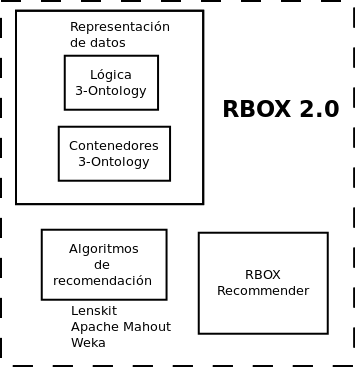
\includegraphics[scale=.6]{images/arquitectura.png}
	\caption{Arquitectura RBOX 2.0 }
	\label{fig:arquitectura}
\end{figure}

RBOX 2.0 se compone de los módulos API y CORE el primero establece la definición de las interfaces y el segundo una implementación para la construcción de SR. En la Figura \ref{fig:diagramapaquetes} se presenta un diagrama de paquetes de RBOX 2.0 con sus dos módulos principales y sub-módulos.

\begin{figure}[tp]
	\centering
	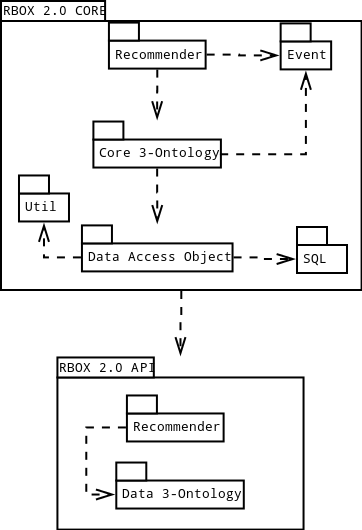
\includegraphics[scale=.6]{images/arquitectureRBOX2.png}
	\caption{Diagrama de paquetes de RBOX 2.0 }
	\label{fig:diagramapaquetes}
\end{figure}

\subsection{RBOX 2.0 API}

Corresponde a la definición de las interfaces  que permiten la representación de datos \textit{(data 3-ontology)} y construcción de  \textit{(recommender)}. Este módulo se compone de los siguientes sub-módulos:

\begin{itemize}
	\item \textbf{Recommender}: corresponde a la definición de las interfaces que permiten construir un recomendador.
	\item \textbf{Data 3-Ontology}: corresponde a la definición de las interfaces que representan los contenedores de sentido y la lógica de la \textit{3-Ontology}.
\end{itemize}

\subsection{RBOX 2.0 CORE}

Corresponde a una implementación del API y un conjunto de módulos que permiten construir un SR. Este módulo se compone de los siguientes sub-módulos:

\begin{itemize}
	\item \textbf{Recommender}: provee una implementación de las interfaces de recomendación.
	\item \textbf{Event}: implementación de componentes para la representación de distintos tipos de eventos.
	\item \textbf{Core 3-Ontology}: componentes que describen el comportamiento del \textit{framework 3-ontology}.
	\item \textbf{Utils}:  componentes utilitarios como por ejemplo de lectura de archivos. 
	\item \textbf{Data access object}: definición e implementación de los componentes DAO definidos.
	\item \textbf{SQL}: definición e implementación de componentes para el acceso a base de datos relacionales mediante JDBC.
	\end{itemize}

\section{Diseño de clases de RBOX 2.0}

En esta sección se realiza la definición de las clases utilizadas que representan el modelo propuesto en el capítulo \ref{capitulo:modelo}.

\subsection{Contenedores de sentido}

La \textit{3-ontology} define tres contenedores de sentido eventos, comunidades y lugares. Cada uno de estos conceptos es representado mediante una interfaz para proveer la flexibilidad y extensibilidad requerida por los SR. Por otro lado, se presentan las representaciones de dos conceptos básicos para un SR como son el usuario e ítem.

En el código \ref{cod:event} se presenta la definición de la  interfaz que representa a un evento que puede ser extendida a nuevos tipos de eventos dado que el valor es de tipo genérico. Se proveen implementaciones para dos eventos interactivos y sociales:

\begin{itemize}
	\item \textbf{Rating}: en este caso el valor es de tipo real bajo un dominio determinado.
	\item \textbf{Tagging}: en este caso el valor es una cadena de caracteres (\textit{String}).
\end{itemize}


\begin{lstlisting}[float, caption = Interfaz Event, label = cod:event]
public interface Event {

   long getUserId();

   long getItemId();

   long getTimestamp();
dos
   long getPlaceId();

   long getCommunityId();  

   <T> T getValue();
}
\end{lstlisting}

 En el código \ref{cod:community} se muestra la definición de la interfaz que representa a una comunidad. Esta hereda de \textit{List} y se compone de usuarios. Un usuario puede explícitamente indicar su pertenencia a una comunidad implícitamente o se puede deducir dado su perfil e historial de eventos. 

\begin{lstlisting}[float, caption = Interfaz Community, label = cod:community]
public interface Community extends List<User>{  

    long getId();

    String getName();
   
    LongSet getUserIds();
}
\end{lstlisting}

En el código \ref{cod:place} se muestra la definición de la interfaz que representa a un lugar. Esta hereda de \textit{List} y se compone de ítems. Un lugar corresponde al espacio físico y/o virtual donde habitan los ítems y son realizados los eventos. 

\begin{lstlisting}[float,caption = Interfaz Place, label = cod:place]
public interface Place extends List<Item> {   

    long getId();
  
    String getName();

    LongSet getItemIds();  
}
\end{lstlisting}

Un usuario es el protagonista de un evento, pertenece a una o varias comunidades. La definición propuesta en este trabajo identifica al usuario en la interfaz del código \ref{cod:user}.

\begin{lstlisting}[float,caption = Interfaz User, label = cod:user]
public interface User {

    long getId();

    String getName();

    LongSet getCommunityIds();
}
\end{lstlisting}

En el código \ref{cod:item} se muestra la interfaz que representa a un ítem. Este corresponde al objeto que es valorado por un usuario y puede habitar uno y/o varios lugares. 

\begin{lstlisting}[float, caption = Interfaz Item, label = cod:item]
public interface Item {

    long getId();

    String getName();

    String getContent();

    LongSet getPlaceIds();
}
\end{lstlisting}

\section{Diseño de una capa de acceso a datos}

El diseño aplicado para representar la \textit{3-Ontology} se constituye de 3 capas lógicas (\textit{tiers}) presentadas en la Figura \ref{fig:capadatos}, la primera consiste en repositorios de datos donde se almacena la información relacionada a los 3 contenedores de sentido de la \textit{3-Ontology} (lugares, eventos y comunidades). Sobre estos repositorios de datos se construye un conjunto de operaciones de acceso a los datos. Esto permite obtener de forma unificada los eventos, lugares, comunidades y relaciones existentes entre ellos. Finalmente, se construye una capa de lógica que permite situar los eventos.

\begin{figure}[tp]
	\centering
	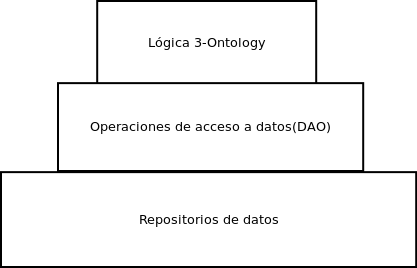
\includegraphics[scale=.6]{images/capadedatos.png}
	\caption{Capa de datos de RBOX 2.0 }
	\label{fig:capadatos}
\end{figure}

\begin{itemize}
\item \textbf{Repositorios de datos}: corresponde a un conjunto de repositorios que pueden contener información de utilidad para los SR.
\item \textbf{Operaciones de acceso a datos}: proveen un acceso a los datos almacenados dentro de múltiples repositorios. Dado que la capa es construida con el patrón DAO se provee abstracción al tipo de repositorio de datos usado.
\item \textbf{Lógica 3-Ontology}: provee un conjunto de operaciones que permiten obtener información relevante para las distintas fases de construcción de un SR.
\end{itemize}

\subsection{Alternativas de solución para distintos tipos de repositorios de datos}

Los repositorios donde están albergados los datos de relevancia de los SR pueden estar dispersos en distintas plataformas, por ejemplo: los datos referentes a las transacciones de los usuarios pueden estar albergadas en una base de datos de análisis (OLAP). Por otro lado, se puede realizar consultas de información referente a las preferencias de sus usuarios dentro de las redes sociales y almacenar en algún repositorio, también se pueden obtener datos geo-localizados de interacciones que los usuarios realicen en alguna aplicación móvil.

A continuación se presentan dos esquemas posibles de solución dependiendo de las necesidades de construcción de un SR.

En un primer esquema se asume que la información proviene de distintos repositorios que pueden ser bases de datos relacionales, objetuales, analíticas, archivos de texto, xml, etc. Cada uno de estos repositorios tiene información referente a los tres contenedores de la \textit{3-ontology} eventos, comunidades y lugares. En este caso, basta solo con implementar la capa \textbf{DAO} para los repositorios específicos.  En la Figura \ref{fig:multiplesrepositorios} se observa un diagrama explicitando la arquitectura propuesta. 

\begin{figure}[tp]
	\centering
	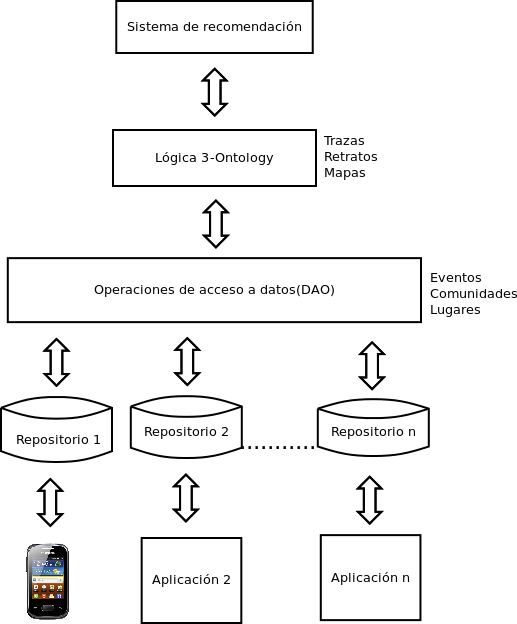
\includegraphics[scale=.6]{images/3-ontology-multiples-repos.png}
	\caption{Múltiples repositorios}
	\label{fig:multiplesrepositorios}
\end{figure}

En un segundo esquema se provee un modelo de datos relacional que es capaz de albergar la información de utilidad de un SR. En este caso se asume que se debe realizar una consolidación de los datos de los diversos repositorios para que sean mapeados dentro de la base de datos relacional de la \textit{3-ontology}. \cite{Molins:2012} provee una herramienta que permite realizar el mapeo desde bases de datos relacionales, archivos de texto y xml al esquema de datos de \textit{Synergy}. En el trabajo futuro expone las directrices para modificar su herramienta y aplicarla a un esquema destino distinto como es el de la \textit{3-ontology}. En la Figura  \ref{fig:unrepositorio} se muestra la arquitectura propuesta para el segundo caso propuesto.

\begin{figure}[tp]
	\centering
	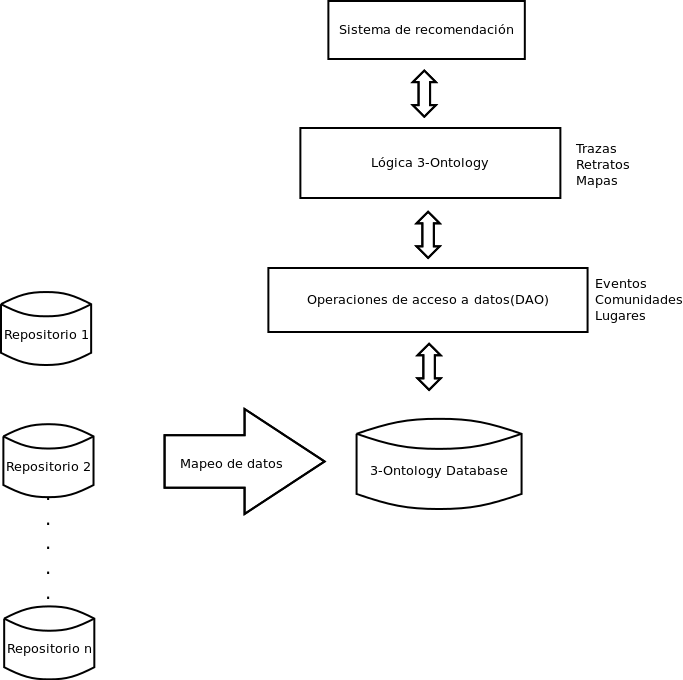
\includegraphics[scale=.6]{images/3-ontology-1-repo.png}
	\caption{Repositorio con la estructura de la \textit{3-Ontology}}
	\label{fig:unrepositorio}
\end{figure}


\subsection{Operaciones de acceso a datos}

Las operaciones de acceso a datos permiten realizar el típico conjunto de operaciones de base de datos \textbf{CRUD} \textit{(Create, Read, Update, Delete)} sobre los eventos, comunidades y lugares. Como ya se mencionó estos pueden estar en distintos repositorios (organizacionales, redes sociales, aplicaciones móviles, etc). Las operaciones de acceso a datos también  permiten obtener información referente a los usuarios e ítems.

El diseño de esta capa se realiza mediante el patrón DAO \textit{(Data Access Object)}\footnote{http://www.oracle.com/technetwork/java/dataaccessobject-138824.html} que permite la abstracción del repositorio de datos. Cada implementación de las interfaces DAO propuestas permitirá el acceso a un repositorio de datos específico. La solución incorpora una implementación genérica para el acceso a una base de datos relacional con el esquema \textit{3-Ontology} mediante JDBC (\textit{Java DataBase Connectivity}).

%El diseño de clases DAO se muestra en la figura x.x
%
%IMAGEN CON EL DISEÑO DE CLASES DAO

Cabe destacar que las operaciones más utilizadas serán de lectura. Sin embargo, las operaciones crear, actualizar y remover pueden ser usadas para un proceso de migrado o para almacenar la información obtenida del proceso de recomendación como por ejemplo nuevas comunidades.

\subsection{L\'ogica de la 3-Ontology}

Como se mencionó en el capítulo \ref{capitulo:modelo} la \textit{3-ontology} se compone de tres formas de representación (trazas, retratos y mapas) que dotan de lógica a los eventos, comunidades y lugares permitiendo obtener las siguientes ventajas:

\begin{itemize}
	\item Representar la composición y recursividad de las comunidades y lugares.
	\item Representar la secuencialidad temporal de los eventos.
	\item Situar a los eventos dentro de una comunidad y lugar.
	\item Representar distintos tipos de interacciones hacia los ítems.
	\item Representar la pertenencia de los ítems y usuarios a un lugar físico y/o virtual.
	\item Representar la pertenencia de usuarios a una o varias comunidades.
	\item Representar la pertenencia entre comunidades y lugares.
\end{itemize}

La representación más un conjunto de métodos permite dar una implementación a la \textit{3-Ontology}. El conjunto de los métodos y la representación son denominados lógica de la \textit{3-Ontology}.

Las trazas denotan la relación existente entre los eventos. Además, de los métodos sobre la causalidad temporal de los eventos se proveen métodos que permiten obtenerlos dadas las características propias de estos para el caso de los SR. Dado lo anterior, se expone un conjunto de métodos dentro de una interfaz que representan a una traza basado en el modelo propuesto. En el código \ref{cod:trace} se muestra la interfaz propuesta para una traza. Los eventos pueden ser obtenidos de forma ordenada mediante el uso de comparadores. Además, los métodos propuestos permiten realizar apoyo a operaciones de pre y post filtrado en CARS obteniendo sólo los eventos relevantes para el cálculo de la recomendación dado un contexto. 

\begin{lstlisting}[float, caption = Interfaz Trace, label = cod:trace]
public interface Trace{

    List<Event> getEvents();

    List<Event> getEvents(Comparator<Event> comparator);

    <E extends Event> List<E> getEvents(Comparator<Event> comparator, Class<E> type);

    <E extends Event> List<E> getEvents(Class<E> type);

    List<Event> getEventsForItem(long itemId);

    List<Event> getEventsForItemByTimestamp(long itemId, long timestamp1, long timestamp2);

    List<Event> getEventsByTimestamp(long timestamp1, long timestamp2);

    <E extends Event> List<E> getEventsForItem(long itemId, Class<E> type);

    <E extends Event> List<E> getEventsForItem(long itemId,Comparator<Event> comparator, Class<E> type);

    List<UserHistory<Event>> getEventsByUser();

    UserHistory<Event> getEventsForUser(long userId);

    UserHistory<Event> getEventsForUserByTimestamp(long userId, long timestamp1, long timestamp2);

    <E extends Event> UserHistory<E> getEventsForUser(long userId, Class<E> type);

    LongSet getUsersForItem(long item);

    <E extends Event>  LongSet getUsersForItem(long itemId, Class<E> type);  

    LongSet getItemsForUser(long userId);

    <E extends Event>  LongSet getItemsForUser(long userId, Class<E> type);
}
\end{lstlisting}

Los retratos representan las relaciones existentes entre las comunidades. Se proveen métodos que permiten obtener información referente a las relaciones entre usuarios y comunidades. Por ejemplo, se puede determinar a que comunidades pertenece el usuario $u$. En el código \ref{cod:portrait} se presenta la definición de la interfaz propuesta para un retrato.

\begin{lstlisting}[float,caption = Interfaz Portrait, label = cod:portrait]
public interface Portrait{
    
    Community getAllUsers();
    
    List<Community> getCommunities();

    <E extends Community> List<E> getCommunities(Class<E> type);

    List<Community> getCommunitiesForUser(long userId);

    <E extends Community> List<E> getCommunitiesForUser(long userId, Class<E> type);  
}
\end{lstlisting}

Los mapas representan las relaciones existentes entre los lugares. Se proveen métodos que permiten obtener información referente a a las relaciones entre los ítems y lugares. Por ejemplo, se pueden obtener todos los lugares a los que un ítem $c$ pertenece. En el código \ref{cod:map} se presenta la definición de la interfaz propuesta para un mapa.

\begin{lstlisting}[float, caption = Interfaz Mapa, label = cod:map]
public interface Map {  
  
    Place getAllItems();
    
    List<Place> getPlaces();
    
    <E extends Place> List<E> getPlaces(Class<E> type);
    
    List<Place> getPlacesForItem(long itemId);

    <E extends Place> List<E> getPlacesForItem(long itemId, Class<E> type);  
}
\end{lstlisting}

\section{Modelo entidad-relación para la 3-Ontology}

Para permitir una representación al nivel de repositorio de datos se provee un modelo entidad-relación que permite realizar un almacenamiento en una base de datos
relacional. En la Figura \ref{fig:modeloentidadrelacion} se muestran las entidades fundamentales (contenedores de sentido) mediante las tablas \textit{Event}, \textit{Community} y \textit{Place}. Los ítems y usuarios son reflejados por las tablas \textit{Item} y \textit{User}.

\begin{figure}[tp]
	\centering
	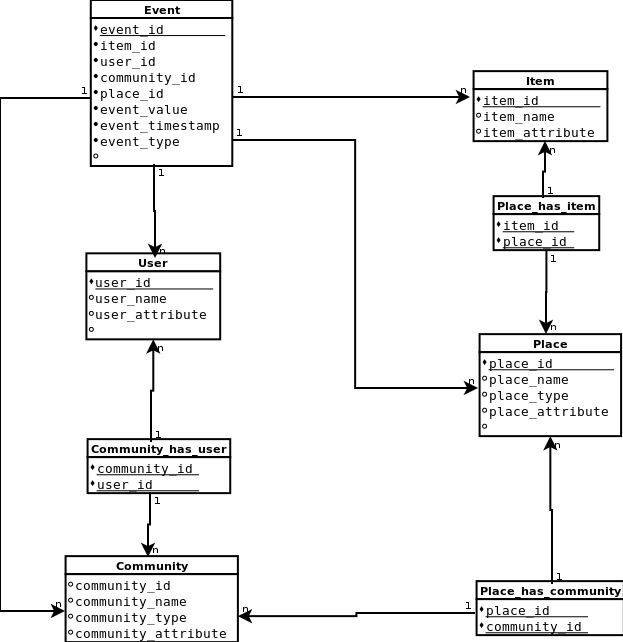
\includegraphics[scale=.6]{images/modeloentidadrelacion.png}
	\caption{Modelo entidad-relación }
	\label{fig:modeloentidadrelacion}
\end{figure}

La columna "\textit{event\_type}" de la tabla \textit{event}  permite modelar varios tipos de interacciones sobre el mismo ítem. En el modelo físico todas las relaciones n-arias del diagrama entidad-relación son reflejadas mediante las siguientes tablas:

\begin{itemize}
	\item \textit{Place\_has\_item}
	\item \textit{Place\_has\_community}
	\item \textit{Community\_has\_user}
\end{itemize}

Estas tablas permiten situar los eventos, usuarios e items en un contexto temporal, espacial y social. El modelo presenta pocos atributos obligatorios para no restringir la representación de los repositorios de datos que no poseen todos los datos necesarios del modelo propuesto. De esta manera, se puede instanciar este modelo de datos para un dominio específico y agregar los atributos que se consideren relevantes. Los únicos atributos obligatorios del evento son el identificador del usuario, objeto, valor y el tipo del evento. Por lo tanto, en las otras tablas solo los identificadores son obligatorios dotando de flexibilidad de representación al modelo propuesto.

\section{Construcción de un SR}
\label{sec:consSR}

Para construir SR en RBOX 2.0 se define la interfaz \textit{RBOXRecommender} (véase el código \ref{cod:recommender}) que permite prestar servicios de recomendación. Los métodos definidos reciben distintos parámetros de entrada para realizar el cálculo de la recomendación para el usuario activo. La salida es una lista de \textit{ScoredItem} que corresponden a ítems con un puntaje calculado por un algún algoritmo de recomendación. Se recomiendan los ítems que tienen el puntaje mayor.

\begin{lstlisting}[float, caption = Interfaz RBOXRecommender, label = cod:recommender]
public interface RboxRecommender {
	
    String getName();
    
    List<ScoredItem> recommend(long idUser, int n);
    
    List<ScoredItem> recommend(long idItem); 
    
    List<ScoredItem> recommend(long idUser, int n,  List<Item> candidates,
    		List<Item> exclude);
    
    List<ScoredItem> recommend(long idUser, List<Item> candidates);
}
\end{lstlisting}

El método definido para construir un SR basado en el modelo propuesto se presenta en la Figura \ref{fig:procesoconstruccionSR}. Primero se deben seleccionar los repositorios de datos que disponen de datos relevantes. Una vez identificados se debe modelar los contenedores de sentido del modelo, en otras palabras se determina que como serán los eventos, comunidades y lugares. Luego se debe determinar si se consolidarán los datos usando la base de datos relacional o implementar la capa \textbf{DAO} para cada repositorio. Una vez que se dispone de los datos, se debe seleccionar un algoritmo de recomendación o de aprendizaje de máquina desde algún API como \textit{Lenskit}, \textit{Weka}, \textit{Apache Mahout} o \textit{Mallet}. Si el algoritmo no cumple con las expectativas se puede modificar y/o cambiar por otro. Finalmente, se implementa la interfaz \textit{RBOXRecommender} utilizando las trazas, retratos y mapas como entrada de datos. Es importante señalar que durante el desarrollo del algoritmo de recomendación se procesan las distintas características provistas por el modelo propuesto.

\begin{figure}[tp]
	\centering
	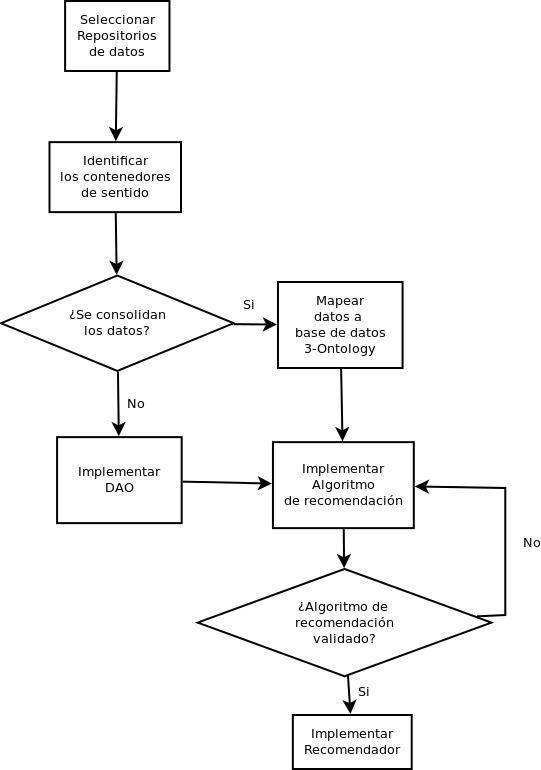
\includegraphics[scale=.6]{images/procesoconstruccionSR.png}
	\caption{Flujograma de creación de un SR }
	\label{fig:procesoconstruccionSR}
\end{figure}

\section{Habilidades necesarias desarrollar con RBOX 2.0}

En esta sección se definen el conjunto de habilidades y conocimientos que debe tener un desarrollador para implementar SR con RBOX 2.0.

\begin{itemize}
\item{\textbf{Lenguaje de programación}}: el desarrollador debe poseer un nivel intermedio del lenguaje de programación \textit{Java}. Esto quiere decir que debe tener conocimiento en:
\begin{itemize}
\item Fundamentos de programación.
\item Uso de interfaces y clases abstractas.
\item Colecciones.
\item Anotaciones.
\item Tipos genéricos.
\item Utilización de librerías.
\end{itemize}

\item{\textbf{Diseño orientado a objetos y patrones de diseño}}: el desarrollador debe tener conocimientos intermedios de orientación a objetos (abstracción, polimorfismo, encapsulación y herencia) que le permita extender el sistema. Además, debe tener conocer los patrones de diseño usados del sistema.

\item{\textbf{Control del ciclo de vida del software}}: este conocimiento se refiere al uso de herramientas que apoyen al proceso de compilación, pruebas y despliegue del software. En el caso de RBOX 2.0 se utiliza \textit{Gradle}, este conocimiento es opcional debido a que se pueden construir SR sin el uso de este tipo de herramientas. 

\item{\textbf{Minería de datos y aprendizaje automático}}: Se asume que el desarrollador tiene conocimientos de técnicas de minería de datos y aprendizaje automático que le permiten construir algoritmos de recomendación. Por ejemplo como se específico en la sección 2.1, los SR basados en \textit{rating} se basan en un problema de predicción, luego el desarrollar debe conocer las técnicas del aprendizaje de máquina disponibles para abordar el problema de predicción.

\end{itemize}

\section{Integración con otras aplicaciones}

La solución provista permite la construcción de SR en \textit{Java} que pueden ser utilizados por aplicaciones Web o móviles que soporten el uso de servicios del tipo \textit{RESTful}. Para lo anterior, se debe encapsular el SR usando \textit{JavaEE 6}\footnote{Java Enterprise Edition 6}, permitiendo así disponer del SR en un contenedor.

Los pasos sugeridos para la construcción son los siguientes:

\begin{enumerate}
\item Construir un SR con el modelo propuesto en este trabajo.
\item Construir un \textit{SessionBean} (\textit{Enterprise Java Bean}) de tipo \textit{Stateless} que encapsule en métodos de negocio la interfaz de recomendación propuesta por RBOX 2.0.
\item Construir servicios de tipo \textit{RESTful} a partir del \textit{SessionBean} creado.
\item Desplegar los servicios en un contenedor dentro de un servidor de aplicaciones.
\item Consumir los servicios desde aplicaciones clientes.
\end{enumerate} 

Esta integración requiere que el desarrollador conozca de arquitectura de aplicaciones empresariales en específico JavaEE, luego implementar la integración sugerida no puede ser aplicada por un desarrollador que no tenga experiencia.


\section{Comparación con otras herramientas}

En esta sección se realiza una comparación de RBOX 2.0 con otras herramientas de software que permiten la construcción de SR. 

RBOX 2.0 para soportar las nuevas características de los SR modernos se rige bajo los siguientes principios de diseño:
\begin{itemize}
	\item \textbf{Mantenibilidad}: se refiere al esfuerzo ahorrado para revisar y corregir errores.
	\item \textbf{Flexibilidad}: se refiere al esfuerzo ahorrado para extender y realizar cambios de configuración del sistema.
	\item \textbf{Reusabilidad}: se refiere al esfuerzo ahorrado de reutilizar módulos y/o componentes de software.
	\item \textbf{Escalabilidad}: se refiere a la capacidad del sistema de soportar una calidad de servicio cuando la carga de eventos aumenta.
\end{itemize}

\cite{Ekstrand:2011} presentan \textit{Lenskit}\footnote{http://lenskit.grouplens.org/} un \textit{toolkit} para construir, investigar y estudiar SR de filtrado colaborativo basados exclusivamente en eventos de tipo \textit{rating}. Se enfoca principalmente en resolver las dificultades referentes a la investigación con SR. \textit{Lenskit} se basa en tres objetivos de diseño:

\begin{itemize}
	\item \textbf{Modularidad}: los algoritmos de recomendación se descomponen dentro de varias piezas constituyentes como normalización, funciones de similaridad y reglas de predicción. Varios de los componentes anteriores no son parte de un algoritmo particular. Esta diseñado para ser altamente modular y reconfigurable.
	\item \textbf{Claridad}: se debe mantener un núcleo simple pero con interfaces que provean integración y extensión en sistemas en tiempo real.
	\item \textbf{Eficiencia}:  se prefiere el código claro antes que obscuras optimizaciones. Puede procesar \textit{Movielens 10m} con 10 millones de eventos de tipo \textit{rating}.
\end{itemize}

Las ventajas de \textit{Lenskit} son su modularidad, configurabilidad y  alto rendimiento para trabajar con SR de filtrado colaborativo. La principal desventaja es no proporcionar una forma estándar de representar los datos que permita modelar características contextuales de las interacciones. Cabe señalar que los algoritmos de filtrado colaborativo utilizados en RBOX 2.0 son extraídos de \textit{Lenskit} ya que son escalables y modulares. La mantenibilidad es asegurada mediante el uso de patrones de diseño y orientación a objetos, la flexibilidad mediante el uso de interfaces simples, la reusabilidad mediante el uso de componentes con alta cohesión y bajo acoplamiento, la escalibilidad mediante el uso de estructuras de datos especializadas como \textit{Sparse Vector}. 

\cite{Babar:2010} presentan \textit{Synergy} una herramienta para la creación, ejecución y comparación de diferentes algoritmos de filtrado colaborativo. La idea fundamental de \textit{Synergy} es que los algoritmos de recomendación deben ser reconfigurados o cambiados por otros durante el tiempo.  Las ventajas de \textit{Synergy} son la posibilidad de modelar diversas formas de interacción, la hibridación de algoritmos de filtrado colaborativo y la generación de SR en formato \textit{plug-in}. Su principal dificultad es que no se encuentra disponible el código por lo tanto no se dispone de información referente a las cuatro propiedades sistémicas evaluadas.

% % Referenciar a Salvador

\cite{Cullache:2011} y \cite{Cortes:2013} presentan RBOX 1.0 una herramienta de software para experimentar con SR de filtrado colaborativo inspirado por \textit{Synergy} y \textit{Weka}. El uso excesivo del patrón de diseño ``\textit{Abstract Factory}'' dificulta la mantenibilidad y flexibilidad del código ya que la mayoría de los objetos de la aplicación son creados con este patrón. Respecto a la reusabilidad se logra mediante la agregación de \textit{plug-ins}. La escalabilidad no es resguardada teniendo serios problemas de rendimiento ya que no posee estructuras de datos especializadas como ``\textit{Sparse Vector}''.

 RBOX 2.0 cumple con la mantenibilidad mediante el uso de patrones de diseño y orientación a objetos. La flexibilidad se asegura mediante el uso de interfaces simples que puedan ser extendidas como es el caso de los eventos \textit{ratings} y \textit{taggings}.  La reusabilidad se asegura mediante el diseño de componentes que posean una alta cohesión y bajo acoplamiento. Finalmente, la escalabilidad se asegura mediante el uso de \textit{Lenskit} para algoritmos de SR de filtrado colaborativo y de \textit{Fast-utils}\footnote{http://fastutil.di.unimi.it/} para estructuras de datos complejas. En la tabla \ref{tabla:comparacionotrasherramientas} se muestra un resumen del cumplimiento de las propiedades sistémicas para cada herramienta. Además, los siguientes patrones de diseño, técnicas de programación y librerías apoyan al cumplimiento de los principios de diseño de RBOX 2.0:
 
 \begin{itemize}
 	\item \textbf{Tipos genéricos}: provee la capacidad de re-usar el mismo código para distintas entradas.
 	\item \textbf{Builders}: patrón creacional que permite la construcción de objetos complejos que no siempre disponen de todos los atributos. Es una alternativa del anti-patrón \textit{telescopic constructor}.
 	\item \textbf{Data access object}: patrón estructural que permite la abstracción de los datos.
 	\item \textbf{Dependency Injection}: patrón creacional que permite resolver las dependencias de objetos en tiempo de ejecución y/o compilación.
 	\item \textbf{Fast-utils}\footnote{http://fastutil.di.unimi.it/}:  es un \textit{framework} que extiende de \textit{Java Collections}\footnote{http://docs.oracle.com/javase/tutorial/collections/} y provee mapas, conjuntos, listas y colas con baja utilización de memoria, rápido acceso e inserción.
 	\item \textbf{Preferencia de objetos inmutables}\footnote{http://docs.oracle.com/javase/tutorial/essential/concurrency/immutable.html}: su uso asegura que el estado de un objeto no cambiará después que es construido. Son útiles en el desarrollo de aplicaciones concurrentes.
 \end{itemize}
 
 
\begin{table}[H]
\caption{Comparación con otras herramientas de software}
\label{tabla:comparacionotrasherramientas}
\begin{center}
	\begin{tabular}{|>{\centering\arraybackslash}p{3cm}  | >{\centering\arraybackslash}p{2cm}  |>{\centering\arraybackslash}p{2cm} |>{\centering\arraybackslash}p{2cm} |>{\centering\arraybackslash}p{2cm} |}
	\hline	& \multicolumn{4}{c|}{Herramientas de software} \\	
	
	\hline Propiedad	 				 				& Lenskit  & 
	Synergy & RBOX 1.0 & RBOX 2.0 \\ 
	\hline Mantenibilidad 		 				& X &   &   & X  \\ 
	\hline Flexibilidad 						& X &   &   & X \\ 
	\hline Reusabilidad 						& X &   & X & X \\ 
	\hline Escalabilidad						& X &   &   & X \\ 
	\hline 
	\end{tabular} 
\end{center}
\end{table}

En la tabla \ref{tabla:comparacionotrasherramientas} se puede observar que \textit{Lenskit} al igual que RBOX 2.0 cumplen con las todas propiedades sistémicas evaluadas. Por otro lado, al no tener disponible el código fuente de \textit{Synergy} no se puede determinar si cumple o no con las propiedades evaluadas. En el caso de RBOX 1.0 se intenta utilizar ciertos patrones de diseño para asegurar algunas propiedades, sin embargo el uso inadecuado de patrones de diseño termina limitando la herramienta. Se observa que las propiedades sistemáticas del software RBOX 2.0 y \textit{Lenskit} son idénticas, sin embargo la principal ventaja que posee RBOX 2.0 sobre \textit{Lenskit} está relacionada con la conceptualización proporcionada por el modelo propuesto, que basa su implementación en la \textit{3-Ontology}. Lo anterior logra que RBOX 2.0 sea una herramienta más comprensible que \textit{Lenskit} permitiendo crear rápidamente prototipos para ámbitos empresariales y científicos agregando todas las ventajas presentadas en la sección 3.3. 


%\section{Resumen}
%
%En este capítulo se presentó RBOX 2.0 una herramienta de software basada en el modelo de representación propuesto. Se presentó la arquitectura del software mediante un diagrama de componentes y de módulos del sistema, posteriormente se presentó el diseño de las clases principales que dan sentido al \textit{framework} propuesto. Finalmente, se presentaron herramientas similares y se evaluaron bajo 4 propiedades sistemáticas mantenibilidad, reusabilidad, flexibilidad y escalabilidad. RBOX 2.0 cumple con las cuatro propiedades que le permite ser un software de calidad para la construcción de SR basados en una representación de datos genérico aplicable a diversos dominios de aplicación.


% % Diseño de clases contenedores de sentido y darse-cuenta

% % Módulos de RBOX 2.0

% % Diseño de un modelo entidad-relación para BD

% % Comparación con herramientas similares
